\section{Bubble Sort}
\label{sec:bubble_sort_teo}

O Bubble Sort, também conhecido como "Ordenação por bolha" ou "Ordenação por flutuação", é um dos algoritmos de ordenação mais simples.

Neste algoritmo, são realizadas comparações entre os dados armazenados em um vetor de tamanho \( n \). Cada elemento na posição \( i \) é comparado com o elemento na posição \( i+1 \). Quando a ordenação procurada — seja ela crescente ou decrescente — é encontrada, ocorre uma troca de posições entre os elementos.

O algoritmo executa dois laços principais:

\begin{enumerate}
    \item[\textbf{1.}] O primeiro laço percorre a quantidade de elementos do vetor:
    \begin{verbatim}
    for (j = 1; j <= n; j++)
    \end{verbatim}
    
    \item[\textbf{2.}] O segundo laço, que está dentro do primeiro, percorre da primeira à penúltima posição do vetor:
    \begin{verbatim}
    for (i = 0; i < n - 1; i++)
    \end{verbatim}
\end{enumerate}


\begin{figure}[!ht]
	\centering
	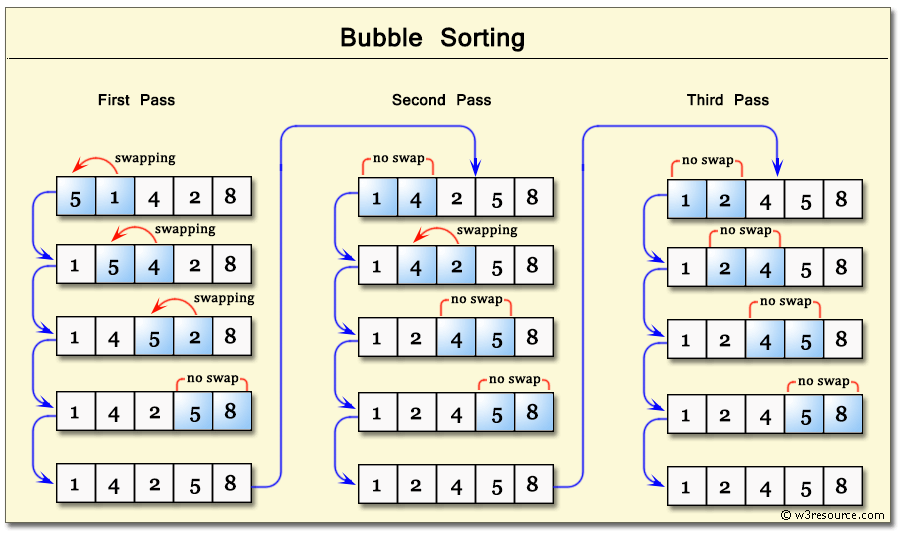
\includegraphics[scale=0.3]{Trabalho-Unidade1-EDB2/latex/figures/bubble/bubbleDiagram.png}
	\caption{Diagrama exemplo de um Bubble Sort}
	\label{fig:merge_sort_example_0}
\end{figure}


\FloatBarrier

\newpage

\subsection{Bubble Sort Iterativo}

\begin{algorithm}
    \caption{Bubble Sort}
    \label{algo:bubble_sort}
    \begin{algorithmic}[1]
        \Require{Lista $A = A_1, A_2, \ldots, A_n$}
        \Ensure{Lista $A$ ordenada}
        \Statex
        \Function{BubbleSort}{$A$}
        \For{$j \gets 1$ to $n - 1$}
            \For{$i \gets 0$ to $n - 2$}
                \If{$A[i] > A[i + 1]$}
                    \State $aux \gets A[i]$ 
                    \State $A[i] \gets A[i + 1]$ 
                    \State $A[i + 1] \gets aux$ 
                \EndIf
            \EndFor
        \EndFor
        \EndFunction
    \end{algorithmic}
\end{algorithm}

\subsubsection{Análise}
Nesse algoritmo, o fator relevante que determina o seu tempo de execução é o número de comparações realizadas. Considerando que o algoritmo foi implementado para um vetor com \( n \) posições, o número de iterações do primeiro laço é \( n \).

O segundo laço possui \( n-1 \) iterações, mas como ele está interno ao primeiro, ele será executado \( n(n-1) = n^2 - n \) vezes. Portanto, podemos dizer que o tempo de execução do algoritmo Bubble Sort, em sua forma iterativa, será \( O(n^2) \), pois:

\[
n^2 - n \leq cn^2, \quad c = 1, \quad n \geq 1
\]

Nesse algoritmo, não há situações melhores ou piores. O comportamento do algoritmo não mudará, independentemente do valor de entrada. Ele realizará todas as comparações, mesmo que desnecessárias.

Além disso, temos que o Bubble Sort será \( \Omega(n^2) \) e \( \Theta(n^2) \), pois:

\[
\lim_{n \rightarrow \infty} \frac{n^2 - n}{n^2} =
\lim_{n \rightarrow \infty} \frac{n - 1}{n} =
\lim_{n \rightarrow \infty} 1-\frac{1}{n} =
1
\]

e 1 \in \mathbb{R}^*_+


\newpage

\subsection{Bubble Sort Recursivo}

\begin{algorithm}
    \caption{Bubble Sort Recursivo}
    \label{algo:bubble_sort_recursivo}
    \begin{algorithmic}[1]
        \Require{Lista $A = A_1, A_2, \ldots, A_n$}
        \Ensure{Lista $A$ ordenada}
        \Statex
        \Function{BubbleSortRecursivo}{$A, n$}
            \If{$n == 1$}
                \Return{}
            \EndIf
            \For{$j \gets 0$ to $n - 2$}
                \If{$A[j] > A[j + 1]$}
                    \State $aux \gets A[j]$
                    \State $A[j] \gets A[j + 1]$
                    \State $A[j + 1] \gets aux$
                \EndIf
            \EndFor
            \State \Call{BubbleSortRecursivo}{$A, n - 1$}
        \EndFunction
    \end{algorithmic}
\end{algorithm}

\subsubsection{Análise}










